\documentclass[5p,final,number,sort&compress]{elsarticle}

\usepackage{lmodern}
\usepackage{textcomp}

\usepackage{graphicx}

\usepackage{ucs}
\usepackage[utf8x]{inputenc}
\usepackage[greek,english]{babel}
\usepackage[LUC,T1]{fontenc}

\makeatletter
\ProvideTextCommandDefault{\textunicodechar}[1]{\uni@char{#1}}
\makeatother

\newcommand{\re}[1]{\texttt{#1}}
\newcommand*{\whack}{\textbackslash}

\usepackage{amsmath}
\usepackage{microtype}
\usepackage{natbib}

\usepackage{tikz}
\usetikzlibrary{calc}
\usetikzlibrary{decorations}
\usetikzlibrary{decorations.pathreplacing}
\usetikzlibrary{matrix}
\usetikzlibrary{positioning}
\usetikzlibrary{shapes.arrows}

\usepackage{xcolor}

\newcommand{\ju}[1]{\textcolor{red}{\footnote{\textcolor{red}{ju: #1}}}}

\newcommand{\todo}[1]{\textcolor{red}{#1}}

\begin{document}
\begin{frontmatter}

\title{Search in a Multi-Encoding World, Or:\\ How I Learned to Stop Worrying and Love Unicode Technical Standard \#18}

\author{Jon Stewart}
\ead{jon@lightboxtechnologies.com}

\author{Joel Uckelman}
\ead{joel@lightboxtechnologies.com}

\address{Lightbox Technologies, Inc. \\ Arlington, VA}

\begin{abstract}
We needed to search a disk image for a pattern, but didn't know how the hits would be encoded. We thought very hard about how to do this. We found an efficient solution.
\end{abstract}

\end{frontmatter}

\section{Introduction}
% in which we say what we will say

\section{Character Encoding Basics}
% in which character encodings are explained

\section{Multipattern Search is Multiencoding Search}
% in which we sketch a general solution to the problem

A \emph{coded character set} is list of pairs, each consisting of a character and the unique integer represeting it, known as a \emph{code point}.  An \emph{encoding} is a method for mapping sequences of code points to sequences of bytes. Examples: Unicode is a coded character set consisting of 1,114,112 code points, intended to be sufficient for representing all text produced by humans. UTF-8 and UTF-16 are encodings capable of representing all Unicode code points as bytes. ASCII, commonly used for simple text files (especially by English speakers), is both a coded character set and an encoding---the 128 code points in ASCII, numbered 0--127, are directly encoded as bytes 0--127. Numerous encodings specific to one or more natural languages were developed---such as Shift\_JIS, EUC-KR, KOI8-R, and ISO 8859-1---which are slowly being supplanted by UTF-8 and UTF-16.

The multiplicity of encodings means that one piece of text can be represented as bytes in numerous ways. E.g., the text ``IRLIBSYR'' can be encoded as in Figure~\ref{fig:enc}.

\begin{figure*}[th]
\centering
\pgfdeclarelayer{background}
\pgfdeclarelayer{foreground}
\pgfsetlayers{background,main,foreground}
\begin{tikzpicture}
  \small
  \matrix (m) [matrix of nodes,nodes in empty cells,nodes={inner sep=0pt,outer sep=0pt,minimum width=5mm},column sep={5mm,between origins},row sep=4ex]
  {
    49 & 52 & 4C & 49 & 42 & 53 & 59 & 52 &    &    &    &    &    &    &    & \\
    49 & 00 & 52 & 00 & 4C & 00 & 49 & 00 & 42 & 00 & 53 & 00 & 59 & 00 & 52 & 00 \\
    C9 & D9 & D3 & C9 & C2 & E2 & E8 & D9 \\
    I  & R  & L  & I  & B  & S  & Y  & R \\
  };

  \draw ([xshift=-2.5mm,yshift=0.5em]m-1-1.north) rectangle ([xshift=2.5mm,yshift=-0.5em]m-1-8.south);

  \foreach \x in {1,...,7}
    \draw ([xshift=2.5mm,yshift=0.5em]m-1-\x.north) -- ([xshift=2.5mm,yshift=-0.5em]m-1-\x.south);

  \draw ([xshift=-2.5mm,yshift=0.5em]m-2-1.north) rectangle ([xshift=2.5mm,yshift=-0.5em]m-2-16.south);

  \foreach \x in {1,...,16}
    \draw ([xshift=2.5mm,yshift=0.5em]m-2-\x.north) -- ([xshift=2.5mm,yshift=-0.5em]m-2-\x.south);

  \draw ([xshift=-2.5mm,yshift=0.5em]m-3-1.north) rectangle ([xshift=2.5mm,yshift=-0.5em]m-3-8.south);

  \foreach \x in {1,...,7}
    \draw ([xshift=2.5mm,yshift=0.5em]m-3-\x.north) -- ([xshift=2.5mm,yshift=-0.5em]m-3-\x.south);

  \node [left=5mm of m-1-1.west] {ASCII and UTF-8};
  \node [left=5mm of m-2-1.west] {UTF16-LE};
  \node [left=5mm of m-3-1.west] {EBCDIC 37};

  \foreach \x in {1,...,16}
    \pgfmathparse{\x-1}
    \pgfmathtruncatemacro{\n}{\pgfmathresult}
    \draw (m-1-1.north -| m-1-\x) node [above=2mm] {\tiny \n};

  \begin{pgfonlayer}{background}
    \foreach \x/\color in {1/red, 2/blue, 3/green, 4/yellow, 5/orange, 6/teal, 7/magenta, 8/cyan}
      \pgfmathparse{2*(\x-1)+1}
      \pgfmathtruncatemacro{\xx}{\pgfmathresult}
      \pgfmathparse{2*\x}
      \pgfmathtruncatemacro{\xxx}{\pgfmathresult}
      \fill [color=\color!30]
        ([xshift=-2.5mm,yshift=0.5em]m-1-\x.north) --
        ([xshift=-2.5mm,yshift=-0.5em]m-1-\x.south) --
        ([xshift=-2.5mm,yshift=0.5em]m-2-\xx.north) --
        ([xshift=-2.5mm,yshift=-0.5em]m-2-\xx.south) --
        ([xshift=-2.5mm,yshift=0.5em]m-3-\x.north) --
        ([xshift=-2.5mm,yshift=-0.5em]m-3-\x.south) --
        ([xshift=2.5mm,yshift=-0.5em]m-3-\x.south) -- 
        ([xshift=2.5mm,yshift=0.5em]m-3-\x.north) --
        ([xshift=2.5mm,yshift=-0.5em]m-2-\xxx.south) --
        ([xshift=2.5mm,yshift=0.5em]m-2-\xxx.north) --
        ([xshift=2.5mm,yshift=-0.5em]m-1-\x.south) --
        ([xshift=2.5mm,yshift=0.5em]m-1-\x.north) --
        cycle;

    \foreach \x/\color in {1/red, 2/blue, 3/green, 4/yellow, 5/orange, 6/teal, 7/magenta, 8/cyan}
      \draw [line width=5mm,color=\color!30,cap=round,join=round]
        (m-1-\x.north) -- (m-1-\x) (m-3-\x) -- (m-4-\x.south);
  \end{pgfonlayer}
\end{tikzpicture}
\caption{Several encodings of the text ``IRLIBSYR''\label{fig:enc}}
\end{figure*}

The UTF-16LE encoding, while containing values similar to the UTF-8 encoding, is twice the length, while the EBCDIC 37 encoding bears no resemblance to the other two. Searching a block of bytes for ``IRLIBSYR'' can mean searching for ``IRLIBSYR'' once for each possible encoding. Hundreds of encodings exist, and while the vast majority of them are obsolete and unlikely to be encountered in data from a contemporary computer, there are still a few dozen which are in common usage. Therefore, if we are trying to establish the existence of a particular string within data for which we don't know the encoding beforehand, the search task can be rather large. Should we need to do this for hundreds, or even thousands of strings (or, in the general case, regular expressions), then it will require a prohibitive amount of time to carry out the search serially, reading the data once for each pattern-encoding pair.

Fortunately, multipattern search rescues us in this situation: Searching in parallel for one string rendered in multiple encodings is structurally the same problem as searching in parallel for multiple strings each rendered in one encoding. Hence, a search for the pattern \texttt{IRLIBSYR.*?SACPOP} in UTF-8, UTF-16LE, UTF-16BE, UTF-32LE, and UTF-32BE does not necessitate five passes over the data (once for each encoding), but merely adds five patterns to the pattern set from which we build our search automaton.

%\PreloadUnicodePage{92}
%\PreloadUnicodePage{182}

%The literals in our regexes are Unicode characters, \emph{not} bytes in a particular Unicode encoding (such as UTF-8). This distinction isn't present when working with traditional ASCII regular expressions, where the characters and the bytes are identical. Distinguishing between characters and bytes in Unicode regular expressions makes the regexes \emph{encoding-independent}, which is a useful property should one wish to search for the same character string in several different encodings.\ju{Example here?} Furthermore, having literals be Unicode characters can improve regex readability over specifying them by code point: While
%\texttt{\textchinesetrad{屁股}} and \texttt{\textchinesetrad{地洞}}
%are easily confusable for those unfamiliar with Chinese, and thus specifying the characters by code point may be called for, of the two patterns matching the Greek name for the city of Athens, even non-Grecophones are likely to prefer \re{\textgreek{Αθήνα}} to \re{\whack x\{0391\}\whack x\{03B8\}\whack x\{03AE\}\whack x\{03BD\}\whack x\{03B1\}}.


\section{Fun With Unicode}
% in which fun is not actually had

Unicode Technical Standard \#18 (hereafter, UTS~\#18) provides guidelines for supporting Unicode characters in regular expressions \citep{uts18}.

% FIXME: missing RL1.2a
% FIXME: also, what happened to RL2.1?

UTS~\#18 defines three levels of support for Unicode in regexes. Level~1, Basic Unicode Support, requires support for specifying Unicode characters by their code points (RL1.1), selectors for Unicode properties (RL1.2), character class union, subtraction, and intersection (RL1.3), simple word boundary matching (RL1.4), simple loose matching (RL1.5), (RL1.6) line boundary matching, and expression of the full range of Unicode characters (RL1.7). Level~2, Extended Unicode Support, requires support for matching cannonical equivalents (RL2.1), extended grapheme clusters (RL2.2), default word boundaries (RL2.3) and name properties (RL2.5), all Unicode properties (RL2.7), as well as support for full default case folding and (RL2.4) and wildcards in property names (RL2.6). Level~3, Tailored Support, requires locale-specific punctuation properties (RL3.1), grapheme clusters (RL3.2), and word boundaries (RL3.3), as well as context (RL3.6) and incremental (RL3.7) matching, the generation of posssible match sets (RL3.9), and match subroutines (RL3.11). We now proceed to explain each of the reqiurements.

\subsection{Level~1: Basic Unicode Support}

%\PreloadUnicodePage{253}

RL1.1 requires Level~1-conformant regex languages to provide a way of specifying code points in hexadecimal. Following PCRE, we meet this requirement with the metacharacter \re{\whack x}, which takes a hexadecimal code point as its argument. E.g., \textsc{latin small letter a} (a) \textsc{arabic ligature sallallahou alayhe wasallam} ( 
%ﷺ
), which is virtually illegible on-screen at 10pt, can be specified as \re{\whack x\{61\}} and \re{\whack x\{FDFA\}}, respectively.

\PreloadUnicodePage{0}

RL1.2 requires Level~1-conformant regex languages to support the character classes defined by the Unicode properties General Category, Script, Alphabetic, Uppercase, Lowercase, White Space, Noncharacter Code Point, Default Ignorable Code Point, Any, ASCII, and Assigned. Unicode properties are fundamentally sets of characters. The General Category and Script properties are multivalued, while the other properties are binary. For example, any given character is either Uppercase or not, while the Script for a letter might be Arabic, Latin, Greek, Cyrillic, or any of 100 other scripts defined in Unicode~6.2.\footnote{For a complete list, see the Unicode~6.2 data file \texttt{PropertyValueAliases.txt} \citep{pva62}.} Following PCRE, we meet this requirement with the metacharacter \re{\whack p}, which takes a Unicode property name (with possible value) as its argument. E.g., \re{\whack p\{Script=Arabic\}} matches any character in Arabic script; \re{\whack p\{General Category=Currency Symbol\}} matches currency symbols such as \$, ¢, \texteuro, and ¥; and \re{\whack p\{White Space\}} matches spaces, tabs, newlines, and carriage returns, as well as more exotic whitespace such as \textsc{mongolian vowel separator}.  \re{\whack p\{Any\}} is the class of all Unicode code points, while \re{\whack p\{Assigned\}} is the class of all code points with a character assigned to them. UTS~\#18 recommends (but does not require) leniency with regard to spaces, case, hyphens, and underscores---which we respect. Hence, \re{\whack p\{Whitespace\}}, \re{\whack p\{wHiTeSpAcE\}}, and \re{\whack p\{\_\_\_white\;\;\;\;space\_\_\_\}} are equivalent. The Unicode Standard defines numerous short forms of properties (such as ``Khmer'' for ``Script=Khmer''), which we also support.

RL1.3 requires Level~1-conformant regex languages to support union, intersection, and set difference on character classes. E.g., one might wish to search for anything Cyrillic or Greek (the union of Cyrillic and Greek scripts), or lowercase Latin letters (the intersection of the Latin letters and the lowercase letters, or, equivalently, the Latin letters minus the uppercase letters). We support only union at present, by permitting \re{\whack p} and other named character classes to appear as members of the bracketed character class construct. \re{[\whack p\{Cyrillic\}\whack p\{Greek\}]} will match any character in either the Cyrillic or Greek scripts. We intend to implement intersection and set difference as part of future work. 

RL1.4 requires Level~1-conformant regex languages to treat all characters having property Alphabetic or Decimal Number as well as the \textsc{zero width non-joiner} and \textsc{zero width joiner} characters as being word characters for the purpose of matching word boundaries, and additionally that combining marks (such as \textsc{combining ring above}) are not separated from their base characters by word boundaries. (A word boundary customarily occurs between any two consecutive characters where one is a word character and the other not, and also at the beginnings and ends of strings. Word boundaries, due to occurring between characters, have zero width.) We do not presently support word boundaries, but doing so is trivial once we add support for positive look-ahead and -behind assertions.

RL1.5 requires Level~1-conformant regex languages to support default case-insensitive matching for all Unicode characters if they support case-insensitive matching at all, and additionally to indicate which properties will be closed under simple default case folding when matching case-insensitively. In order to unpack this requirement, we need to understand default case-insensitive matching, closure, and simple default case folding. Default case-insensitive matching, as defined in \citep[\S 3.1.3]{ustd62}, is too complex to explain here. It suffices to say that the standard defines the function $\operatorname{toCasefold}$ for every string, and two strings $S,T$ are default case-insensitively equivalent iff $\operatorname{toCasefold}(S) = \operatorname{toCasefold}(T)$. Thinking of case-folding as simple lowercasing is fairly close, but misses a few corner cases that the standard handles. In order to fulfil the requirement of RL1.5, a pattern interpreted case-insensitively must match all strings which are case-insensitively equivalent to the strings that same pattern would match case-sensitively. This requirement touches on a feature of Unicode which surprises novices, namely that lowercasing and uppercasing are not inverses. According to the Unicode Standard, both \textsc{latin capital letter k} (K) and the \textsc{kelvin sign} (K) lowercase to \textsc{latin small letter k}, but \textsc{latin small letter k} (k) uppercases to \textsc{latin capital letter k} (K) only.\footnote{Note that in many fonts, the Kelvin sign is indistinguishable from a capital K.} Both \textsc{latin small letter s} (s) and \textsc{latin small letter long s} (
%ſ
) uppercase to \textsc{latin capital letter s} (S), but \textsc{latin capital letter s} lowercases to \textsc{latin small letter s} only.\footnote{You might have seen a long s, also known as a medial s, in books from the 17th century (or fascimilies thereof). E.g., the title page of the 1668 edition of Milton's \emph{Paradise Lost} spells the title as \emph{Paradi
%ſ
e Lo
%ſ
t}.}
A consequence of this is that the character class $\re{[A-Z]}$ matches not 52, but 54 different letters when interpreted case-insensitively in an encoding supporting full Unicode. Now for property closure: Recall that properties can be thought of as sets of characters. Let $C_0$ be a set, $o$ a function from sets to sets, and $C_n = o(C_{n-1}) \cup C_{n-1}$ for $n > 0$. The set which is the closure of $C_0$ under $o$ is the $C_i$ such that $C_i = C_{i+1}$. (And, in fact, if $C_i$ is closed under $o$, then $C_i = C_j$ for all $j \ge i$.) That is, the closure of $C_0$ under $o$ is the set from which no new elements are generated when $o$ is iteratively applied to it. E.g., the set $\{\mathrm{A}\}$ is not closed under simple default case folding because A case-folds to a, and $\mathrm{a} \notin \{\mathrm{A}\}$. The set $\{\mathrm{A}, \mathrm{a}\}$ is closed under simple default case-folding, since A case-folds to a and a case-folds to A. Now it should be clear what it would mean for a Unicode property to be closed (or not) under case-folding when matching case-insensitively. The property General Category=Letter, by virtue of containing all letters, whether upper-, lower- or uncased, cannot fail to be closed under simple default case-folding when matching case-insensitively in any correct implementation, but whether an implementation similarly closes the property General Category=Uppercase Letter is up to the implementers. It would be strange---though permissible---if \re{\whack p\{General Category=Uppercase Letter\}} in a case-insensitive pattern did not match lowercase letters. We chose to close all properties under simple default case-folding when matching case-insensitively, in accordance with the principle of least surprise.

RL1.6 requires Level~1-conformant regex languages to recognize all of LF (U+0A), CR (U+0D), CR LF (U+0A U+0D), NEL (U+85), \textsc{line separator} (U+2028), and \textsc{paragraph separator} (U+2029) as ending logical lines. (LF is the traditional end-of-line character on UNIX, CR LF on Windows, CR on MacOS prior to OS X. Customarily, ASCII regex implementations would recognize some combination of these as line endings, perhaps depending on the platform where they were running.) The start- and end-of-line assertions \re{\^} and \re{\$} are not terribly useful when searching data, such as disk images, which is not line-oriented. Hence, we support RL1.6 vacuously by not supporting line-break assertions at all.

RL1.7 requires Level~1-conformant regex languages to handle all code points, as well as treating UTF-16 surrogate pairs as single code points when matching. In the early days of Unicode, some encoders and decoders balked at valid characters above U+7FF (the last two-byte character in UTF-8) or U+FFFF (the last two-byte character in UTF-16); some UTF-16 decoders also incorrectly decoded surrogate pairs as two invalid code points rather than single valid ones. These two requirement are aimed at heading off such shoddy implementations. We support all code points and correctly interpret UTF-16 surrogate pairs. 

\subsection{Level~2: Extended Unicode Support}

RL2.2 requires Level~2-conformant regex languages to provide a way of matching an any extended grapheme cluster, a literal cluster, and extended grapheme cluster boundaries. An \emph{extended grapheme cluster} is the glyph that from a user's point of view consists of a single character.\footnote{This is a gloss. For the definition, see \citep[\S 3]{uax29}.} E.g., the sequence of the two Unicode characters \textsc{latin small letter o} and \textsc{combining double acute accent} form the extended grapheme cluster \H{o} used in Hungarian (which can also be produced by the single Unicode character \textsc{latin small letter o with double acute}). The metacharacter for matching any extended grapheme clusters is analogous to the dot metecharacter for matching any single code point. PCRE uses \re{\whack X} for this purpose. E.g., on the sequence $\langle \text{o U+030B} \rangle$, the regex \re{.} matches the o, while \re{\whack X} matches the o and its combining accent as a unit. The requirement for matching literal clusters is intended to facilitate including them in character classes, e.g., as in \re{[\H{o}\whack q\{o\whack x\{030B\}]\}} which follows the UTS~\#18 sample syntax and is intended to match either representation of~\H{o}. Support for literal clusters is vexing, as it means that a character class can no longer be expected always to match a single character---in the example, one member of the class is two Unicode characters long, instead of one. We do not yet support any of RL2.2.

RL2.3 requires Level~2-conformant regex languages to provide assertions for matching Unicode default word boundries, as defined in \citep[\S 4]{uax29}. This requirement is far more demanding than simple word boundaries as defined in RL1.4, and we do not presently support it.

RL2.4 requires Level~2-conformant regex languages to provide full default Unicode case folding if they provide case conversion at all. The salient difference between this requirement and that of RL1.3 can be seen for characters like U+DF, \textsc{latin small letter sharp s} (ß). In German, ß capitalizes to SS. This causes common words (e.g., straße) to change length when converted to uppercase (STRASSE). Similar things apply to \textsc{latin capital ligature ij} (
%IJ
), \textsc{latin small ligature ij} (
%ij
), and the sequences IJ and ij, all of which are considered a single letter in Dutch; the digraphs \textsc{latin small letter dz} (
%dz
), \textsc{latin capital letter dz} (
%DZ
), and \textsc{latin capital letter d with small letter z} (
%Dz
), used in some Slavic languages; as well as the various ligatures 
%ff
,
%fi
, 
%fl
, etc.\ used in quality printing. Full default case folding should make the pattern \re{straße} case-insensitively match all of the following: strasse, straße, STRASSE. While this feature is undoubtedly useful, especially for investigators unaware of the subtleties of various languages, the primary difficulty with implementing RL2.4 is the same as with RL2.2, namely that character classes can sometimes contain character sequences in addition to single characters, and as such, we do not yet support it.

RL2.5 requires Level~2-conformant regex languages to support referring to characters by name. Many Unicode characters, such as \textsc{apl functional symbol tilde diaresis} (
%⍨
) and \textsc{pile of poo} ( ), are not easy to type and have descriptive names more memorable than their hexadecimal code points; therefore, being able to specify them by name might on occasion be useful. Following PCRE, we provide the \re{\whack N} metacharacter, which takes the name of a character as its argument and matches the named character, as well as supporting the Name property via \re{\whack p}. E.g., \textsc{thai character tho phuthao} (
%ฒ
) is matched both by \re{\whack N\{thai character tho phuthao\}} and \re{\whack p\{name=thai character tho phuthao\}}.

RL2.6 requires Level~2-conformant regex languages to support wildcards in Unicode property values. The suggested syntax is more expansive, permitting arbitrary regular expressions to appear as property value matchers. For example, \re{\whack p\{name=/l.*tel/\}} would produce a chacter class containing \textsc{byzantine musical symbol apostrofoi telous ichimatos} ( ), \textsc{black telephone} (), and \textsc{love hotel} ( ), among others. We do not yet support this, as we do not yet have a compelling use case for it.

RL2.7 requires Level~2-conformant regex languages to support all (non-provisional, non-contributory, non-obsolete, non-deprecated) Unicode properties. This amounts to several dozen propeties beyond those required by RL1.2, such as Hex Digit, Changes When Lowercased, and Ideographic. We support these properties.

\subsection{Level~3: Tailored Support}

RL3.1 requires Level~3-conformant regex languages to have locale-specific punctuation properties. For example, \textsc{left-pointing double angle quotation mark} («) and \textsc{right-pointing double angle quotation mark} (») might be considered Punctuation in a French locale, but not in an English one.

RL3.2 requires Level~3-conformant regex languages to have locale-specific collation order for collation grapheme clusters. The most striking effect of a locale's collation order on regexes involves ranges in character classes. The standard collation order used for ranges in character classes is ascending code point order. In the standard, locale-agnostic collation the character class \re{[O-P]} matches O and P only, which is correct for many languages---but not for German, which sorts \"O between O and P. (This problem is not solvable simply by declaring that \"O always sorts between O and P, as then the standard collation would be wrong for Swedish, where \"O sorts as the last letter of the alphabet.)  Hence, a regex language conforming to this requirement should provide a collation order which respects the locale selected by the user.

RL3.3 requires Level~3-conformant regex languages to have locale-specific word boundaries. Default word boundaries (RL2.3) are insufficient for splitting words in some languages. Thai, for example, has no interword whitespace, so detecting word boundaries is not a simple matter of looking for alternations between word and non-word characters.

RL3.6 requries Level~3-conformant regex languages to support unmatchable leading and trailing context % TODO 

RL3.7 requires Level~3-conformant regex languages to support incremental matching. % TODO

RL3.9 requires Level~3-conformant regex languages to support the generation of possible match sets for any given pattern. Novice regex users have always been plagued by unexpected matches and nonmatches. With the expansion of regexes to Unicode, the possibility that a given regex could match unexpectedly increases---hence, there is great practical utility in being able to see sample matches for any given pattern, especially if that means correcting a faulty pattern before running an hours- or days-long search. We support generation of possible matches for a pattern by randomly walking its search automaton, reading off a match for each complete branch walked.

RL3.11 requires Level~3-conformant regex languages to permit registration of arbitrary submatching functions. We have no intention of supporting this, as the injection of arbitrary code into our match engine is incompatible with providing performance guarantees.

\subsection{UTS~\#18 Conformance}

\begin{table}
\small
\centering
\setlength{\tabcolsep}{3pt}
\begin{tabular}{l|c|c|c|c|c|}
 \multicolumn{1}{c}{}
 & \multicolumn{1}{c}{\rule{1em}{0pt}\makebox[0cm][r]{\rotatebox[origin=rB]{-45}{lightgrep}}}
 & \multicolumn{1}{c}{\rule{1em}{0pt}\makebox[0cm][r]{\rotatebox[origin=rB]{-45}{ICU 50}}}
 & \multicolumn{1}{c}{\rule{1em}{0pt}\makebox[0cm][r]{\rotatebox[origin=rB]{-45}{Perl 5.6}}}
 & \multicolumn{1}{c}{\rule{1em}{0pt}\makebox[0cm][r]{\rotatebox[origin=rB]{-45}{Java 7}}}
 & \multicolumn{1}{c}{\rule{1em}{0pt}\makebox[0cm][r]{\rotatebox[origin=rB]{-45}{Python regex}}} \\
\hline
Level 1: Basic Unicode Support     & $\circ$   & $\bullet$ & $\circ$   & $\bullet$ & $\bullet$ \\
\hline
RL1.1 Hex Notation                 & $\bullet$ & $\bullet$ & $\bullet$ & $\bullet$ & $\bullet$ \\
RL1.2 Properties                   & $\bullet$ & $\bullet$ & $\bullet$ & $\bullet$ & $\bullet$ \\
RL1.3 Subtraction and Intersection & $\circ$   & $\bullet$ & $\circ$   & $\bullet$ & $\bullet$ \\
RL1.4 Simple Word Boundaries       &           & $\bullet$ & $\bullet$ & $\bullet$ & $\bullet$ \\
RL1.5 Simple Loose Matches         & $\bullet$ & $\bullet$ & $\bullet$ & $\bullet$ & $\bullet$ \\
RL1.6 Line Boundaries              &           & $\bullet$ & $\circ$   & $\bullet$ & $\bullet$ \\
RL1.7 Supplementary Code Points    & $\bullet$ & $\bullet$ & $\bullet$ & $\bullet$ & $\bullet$ \\
\hline
Level 2: Extended Unicode Support  & $\circ$   & $\circ$   & $\circ$   & $\circ$   & $\circ$   \\
\hline
RL2.1 Canonical Equivalents        &           &           &           & $\bullet$ &           \\
RL2.2 Extended Grapheme Clusters   &           & $\circ$   & $\circ$   &           & $\bullet$ \\
RL2.3 Default Word Boundaries      &           & $\bullet$ &           &           &           \\
RL2.4 Default Case Conversion      &           &           &           &           &           \\
RL2.5 Name Properties              & $\bullet$ & $\bullet$ & $\bullet$ &           & $\bullet$ \\
RL2.6 Wildcards in Property Values &           &           &           &           &           \\
RL2.7 Full Properties              & $\bullet$ &           & $\bullet$ &           & $\bullet$ \\
\hline
Level 3: Tailored Support          & $\circ$   &           & $\circ$   &           &           \\
\hline
RL3.1 Tailored Punctuation         &           &           &           &           &           \\
RL3.2 Tailored Grapheme Clusters   &           &           &           &           &           \\
RL3.6 Context Matching             &           &           & $\circ$   &           &           \\
RL3.7 Incremental Matches          &           &           &           &           &           \\
RL3.9 Possible Match Sets          & $\bullet$ &           &           &           &           \\
RL3.11 Submatchers                 &           &           &           &           &           \\
\hline
\end{tabular}

\medskip
$\bullet = $ full support, $\circ = $ partial support
\caption{UTS~\#18 Support\label{tab:uts18-support}}
\end{table}

Table~\ref{tab:uts18-support} summarizes UTS~\#18 conformance for lightgrep, as well as for ICU~50 \citep{icuregex}, Perl~5.6 \citep{perlunicode}, Java~7 \citep{jdk7pattern}, and the Python regex library \citep{pythonregex}.

% FIXME: could add Python regex library

\section{Encoding Chains}

\begin{figure*}[ht]
\centering
\tikzstyle{func} = [draw,rounded corners,minimum width=6mm]
\begin{tikzpicture}[every to/.style={thick,->}]

  \matrix (m) [matrix of math nodes,nodes in empty cells,column sep={10mm,between origins},nodes={outer sep=0pt,minimum height=6mm,anchor=center}] {
    & |[func]| c_0 & |[func]| c_1 & \cdots & |[func]| c_n & |[func]| e & |[func]| b_0 & |[func]| b_1 & \cdots & |[func]| b_n & \\
  };

  \foreach \x in {1,...,10}
    \pgfmathparse{\x+1}
    \pgfmathtruncatemacro{\xx}{\pgfmathresult}
    \path[every edge/.style={draw,semithick,->}] (m-1-\x) edge (m-1-\xx);

  \draw [semithick,decorate,decoration={brace,amplitude=5pt,raise=3pt}] (m-1-5.south east) -- (m-1-2.south west) node [midway,below=8pt,text width=4cm,text centered] {\small code point-code point\\ transformations};

  \draw [semithick,decorate,decoration={brace,amplitude=5pt,raise=3pt}] (m-1-10.south east) -- (m-1-7.south west) node [midway,below=8pt,text width=3cm,text centered] {\small byte-byte\\ transformations};

  \draw [semithick] ([yshift=-3pt]m-1-6.south) -- +(0,-1.25cm) node [below] {\small code point-byte transformation};

\end{tikzpicture}
\caption{An abstract transformation chain\label{fig:abs-chain}}
\end{figure*}


\begin{figure*}[ht]
\centering
\small
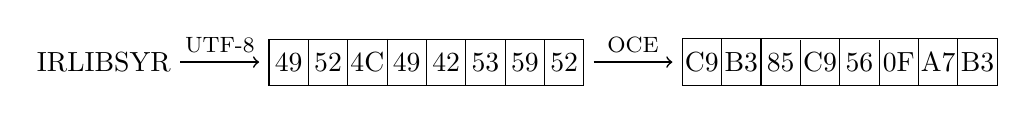
\begin{tikzpicture}
  \node (text) {IRLIBSYR};

  \matrix (utf8) [matrix of nodes,nodes in empty cells,nodes={inner sep=0pt,outer sep=0pt,minimum width=5mm},column sep={5mm,between origins},right=of text]
  {
    49 & 52 & 4C & 49 & 42 & 53 & 59 & 52 \\
  };

  \draw ([xshift=-2.5mm,yshift=0.5em]utf8-1-1.north) rectangle ([xshift=2.5mm,yshift=-0.5em]utf8-1-8.south);

  \foreach \x in {1,...,7}
    \draw ([xshift=2.5mm,yshift=0.5em]utf8-1-\x.north) -- ([xshift=2.5mm,yshift=-0.5em]utf8-1-\x.south);

  \matrix (oce) [matrix of nodes,nodes in empty cells,nodes={inner sep=0pt,outer sep=0pt,minimum width=5mm},column sep={5mm,between origins},right=of utf8]
  {
    C9 & B3 & 85 & C9 & 56 & 0F & A7 & B3 \\
  };

  \draw ([xshift=-2.5mm,yshift=0.5em]oce-1-1.north) rectangle ([xshift=2.5mm,yshift=-0.5em]oce-1-8.south);

  \foreach \x in {1,...,7}
    \draw ([xshift=2.5mm,yshift=0.5em]oce-1-\x.north) -- ([xshift=2.5mm,yshift=-0.5em]oce-1-\x.south);

  \path [every edge/.style={draw,semithick,->}]
    (text) edge node [above] {\footnotesize UTF-8} (utf8)
    (utf8) edge node [above] {\footnotesize OCE} (oce);

\end{tikzpicture}
\caption{The chain \texttt{UTF-8|OCE} applied to text ``IRLIBSYR''\label{fig:concrete-chain}}
\end{figure*}

Character encodings are a special case of something more general. Character encodings map (sequences of) code points to sequences of bytes. One could also imagine transformations which map (sequences of) code points to (sequences of) code points, and sequences of bytes to sequences of bytes, and that such transformations could be chained together, as in Figure~\ref{fig:abs-chain}. (\emph{Composed} would be the mathematical term here.) For example, Caesar ciphers (a.k.a.\ monoalphabetic substitution ciphers) can be thought of as maps from bytes to bytes. It is not far-fetched to think that one might want to search for text which is both encoded and transformed in one of these additional ways.

A prime example of this is Outlook Compressible Encryption, which, despite its name, is just a Caesar cipher applied to mailboxes used by Microsoft's ubiquitous Outlook email client. If you are thinking that this provides no real security because Caesar ciphers are easily defeated by frequency analysis, you would be correct---nonetheless, OCE is an impediment to searching Outlook mailbox files, since it changes the byte patterns contained therein. This forces the investigator either to hand-adjust patterns to account for OCE (which requires knowledge of both the target character encoding and OCE), or to decypher the OCE'd portions of Outlook mailboxes before searching them (which works only if you know you have such files, and probably not on deleted mailbox fragments in a drive's slack space). A better solution---one which we have implemented---generalizes specifying multiple encodings for each pattern by letting the user specify one or more \emph{transformation chains} per pattern. Continuing with the example above, specifying the chain \texttt{UTF-8|OCE} on the pattern \texttt{IRLIBSYR} would cause the byte sequence searched for to be UTF-8-encoded, then OCE'd, as seen in Figure~\ref{fig:concrete-chain}, thus permitting us to search for hits for this pattern in OCE'd Outlook mailboxes directly, without any human expertise required.

\section{Interpreting Hits in Context}
% in which we describe issues with decoding hit context

\section{Conclusion}
% in which we say what we have said

\bibliographystyle{elsarticle-num}
\bibliography{enc}

\end{document}
